\section{Interacción de un robot móvil con su entorno}
El entorno o mundo en el que opera un robot se define por su estado, que engloba las condiciones y características tanto del robot mismo como del entorno circundante. Sin embargo, en la práctica, especificar un estado completo es prácticamente imposible para cualquier sistema robótico realista. Esto se debe a que un estado completo abarcaría no solo todos los aspectos del entorno que podrían tener un impacto en el futuro, sino también las propias características y estados internos del propio robot. Por lo tanto, en las implementaciones prácticas se selecciona un pequeño subconjunto de todas las variables de estado para formar un estado representativo y manejable. Esta selección incluye variables como \cite{thrun_probabilistic_2005}: 
\begin{itemize}
	\item La pose del robot: Comprende su ubicación y orientación con respecto a un marco de coordenadas global. Para un robot móvil en un entorno plano, la pose suele estar constituida por sus dos coordenadas de ubicación en el plano y su orientación de giro (\textit{yaw}) \cite{thrun_probabilistic_2005}.
	\item La velocidad del robot: En un entorno plano, las velocidades críticas para un robot móvil de dos ruedas son la velocidad lineal y la angular. La velocidad lineal indica cuán rápido avanza el robot en línea recta a lo largo de su trayectoria, mientras que la velocidad angular determina la rapidez con la que el robot gira alrededor de su centro de giro. Esta última se regula ajustando las velocidades angulares de las ruedas izquierda y derecha \cite{thrun_probabilistic_2005}.
	\item La ubicación y características de los objetos circundantes  en el entorno: Este aspecto abarca características como la apariencia visual de objetos, su forma, tamaño, disposición espacial y cualquier otra propiedad relevante para la interacción del robot con su entorno. Estas variables son cruciales para interpretar y comprender la situación del robot en distintos escenarios \cite{thrun_probabilistic_2005}.  
\end{itemize}

Además de lo anterior, se distinguen dos tipos fundamentales de interacciones entre un robot y su entorno: la influencia del robot en el estado mediante acciones de control de sus actuadores y la recopilación de información del estado a través de los sensores del propio robot. Las acciones de control, como el movimiento del robot y la manipulación de objetos, provocan cambios instantáneos en el estado del entorno lo que demanda una continua adaptación y respuesta por parte del sistema robótico para actualizar las condiciones del mismo. Por otro lado, se utilizan los sensores para capturar información sobre el estado del entorno. Sin embargo, es común que las mediciones de los sensores tengan cierto retraso, por lo que proporcionan una percepción del estado en momentos relativamente anteriores \cite{thrun_probabilistic_2005}. 

\begin{figure}[H]
	\centering
	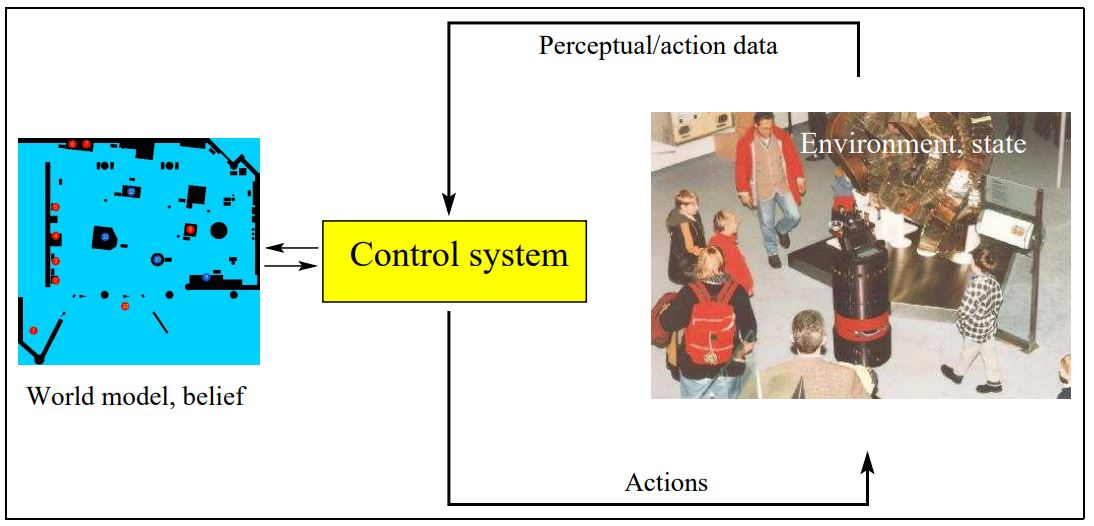
\includegraphics[width=0.7\textwidth]{inter_ent.jpg}
	\caption{Interacción de un robot con su entorno \cite{thrun_probabilistic_2005}.}
	\label{fig:interaccion_ent}
\end{figure}

\section{Modelos probabilístico de movimiento para robots móviles en entornos planos}
Los modelos probabilísticos de movimiento son empleados en robótica móvil para estimar la posición futura de un robot en función de su movimiento y de las incertidumbres asociadas que puedan influir en su trayectoria como la imprecisión de los sensores, la presencia de fuerzas externas, el ruido, entre otros. Un enfoque comúnmente utilizado es el modelo de movimiento de velocidad, el cual se basa en la relación entre las velocidades lineales y angulares del robot y su ubicación actual en el espacio para predecir su posición futura. Esta metodología en particular ofrece ventajas significativas como su facilidad de implementación y simplicidad para predecir, de manera directa, el movimiento futuro del robot en entornos simples y controlados \cite{thrun_probabilistic_2005}.

Por otro lado, se pueden emplear las mediciones de odometría como base para calcular el movimiento del robot a lo largo del tiempo. La odometría es una técnica utilizada en navegación para estimar la posición y desplazamiento de un vehículo móvil por medio de de la medición de las distancias recorridas por sus ruedas o sistemas de locomoción. Este enfoque, conocido como modelo de odometría, integra la información de los encoders en las ruedas para medir la rotación de las mismas y calcular la distancia recorrida. Estas mediciones combinadas con otros datos de orientación son empleados para estimar la posición actual del robot. Sin embargo, este método sufre de errores acumulativos a medida que el robot se desplaza debido a pequeñas desviaciones en la rotación de las ruedas \cite{thrun_probabilistic_2005}. 

Alternativamente, existe un modelo más complejo, que considera la cinemática del robot con la geometría del mismo. El modelo de movimiento cinemático considera la velocidad lineal y angular del robot, junto con la forma y tamaño del mismo para predecir con precisión el desplazamiento y la orientación futura del robot. Este enfoque destaca por su capacidad para capturar el comportamiento del robot en el espacio, ofreciendo una representación más completa del movimiento. Además, su consideración en la geometría proporciona un análisis más profundo en cómo el diseño del robot influye en su movimiento \cite{fahimi_autonomous_2009}.

\section{Robot móvil con tracción diferencial}
Los robots móviles con ruedas (WMRs, por sus siglas en inglés) están compuestos por uno o más cuerpos rígidos equipados con un sistema de locomoción. En términos generales, constan de un cuerpo rígido que funciona como base o chasis, junto con un conjunto de ruedas que les permite moverse sobre el suelo. En un robot móvil de tracción diferencial existen dos ruedas fijas con un eje de rotación común y orientación constante, las cuales se controlan de manera independiente para imponer diferentes valores de velocidad angular y controlar el movimiento lineal del propio robot. Además, estos robots pueden contar con una o más ruedas giratorias de apoyo no motorizadas para proporcionar estabilidad adicional. Es importante destacar que un robot de este tipo puede realizar giros en su propio eje sin necesidad de desplazarse, siempre que las velocidades angulares de las dos ruedas sean iguales y opuestas \cite{siciliano_robotics_2009}. 

En robótica móvil con sistemas de ruedas, se emplea la cinemática diferencial para establecer la relación entre las velocidades de las ruedas del robot y su movimiento en el espacio cartesiano. De esta manera, así como cada rueda contribuye al movimiento general del robot, estas imponen restricciones específicas a la velocidad del mismo. En el caso particular de un robot móvil con tracción diferencial y ruedas fijas, operando en un entorno plano, cada rueda se desplaza únicamente en el plano que la contiene, lo que implica la ausencia de deslizamiento relativo entre la rueda y la superficie, y garantiza que no se produzcan deslizamientos laterales. Estas restricciones, conocidas como restricción de rodadura y restricción de deslizamiento, son fundamentales para definir el modelo cinemático del robot como \cite{multi-robot_nodate}:

\begin{equation}
	\label{eq:mod_cine1}
	\dot{x_b}\cos{\theta}+\dot{y_b}\sin{\theta}=\dfrac{D_{L}\dot{\theta_{L}}+D_{R}\dot{\theta_{R}}}{4}
\end{equation}
\begin{equation}
	\label{eq:mod_cine2}
	\dot{x_b}\sin{\theta}+\dot{y_b}\cos{\theta}=0
\end{equation}
\begin{equation}
	\label{eq:mod_cine3}
	2l\dot{\theta}=D_{R}\dot{\theta_{R}}-D_{L}\dot{\theta_{L}}
\end{equation}

donde $(x_{b},y_{b})$ es la coordenada del centro de masa del robot, $\dot{x_b}$ e $\dot{y_b}$ son las velocidades del centro de masa a lo largo de los ejes $X_R$ y $Y_R$, correspondiente al sistema local de referencia del robot, donde el eje longitudinal $X_R$ apunta hacia adelante en la dirección del movimiento del robot y $Y_R$ es perpendicular al eje longitudinal apuntando hacia la izquierda del robot. $\theta$ representa la orientación del robot respecto de su posición inicial en el punto de inicio del movimiento y $\dot{\theta}$ corresponde a la velocidad angular en el sistema del robot. $D_R$ y $D_L$ son los diámetros nominales de las ruedas derecha e izquierda. Las velocidades angulares de cada rueda se denotan por $\dot{\theta_{R}}$ y $\dot{\theta_{L}}$. La distancia nominal entre las dos ruedas se representa por $l$ \cite{multi-robot_nodate}.

\begin{figure}[H]
	\centering
	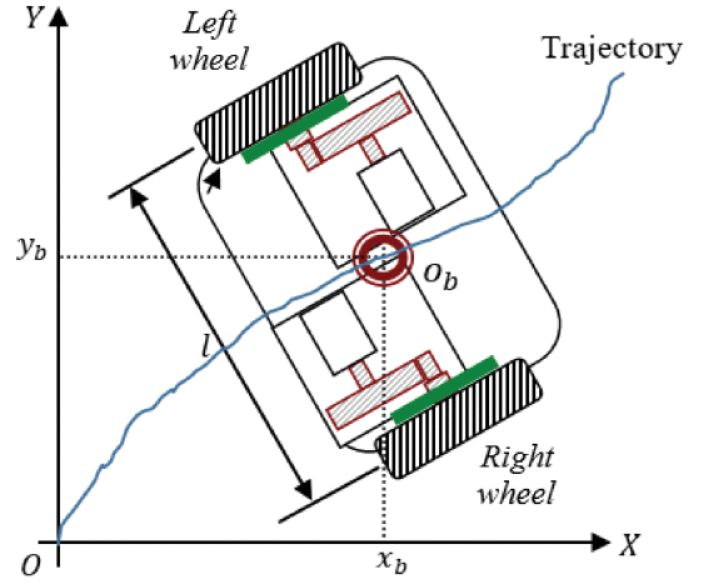
\includegraphics[width=0.6\textwidth]{mob_rob_coo_sys.jpg}
	\caption{Sistema de coordenadas de referencia de un robot móvil con tracción diferencial. $XOY$ muestra el marco de referencia mundial.$(x_{b},y_{b})$ es la coordenada del centro de masa del robot a lo largo de los ejes $X_R$ y $Y_R$, los cuales representan el sistema local de coordenadas del robot \cite{multi-robot_nodate}.}
	\label{fig:coordenadas_rob_mob}
\end{figure}

\section{Localización de robots móviles}
En términos de percepción del entorno, la localización de robots móviles constituye uno de los desafíos fundamentales en la robótica. Este desafío se enfoca en determinar la pose de un robot con respecto a un mapa predefinido del entorno en el que opera. Esta información es crucial para permitir que los robots móviles ejecuten tareas autónomas de manera efectiva, tales como la navegación, manipulación de objetos o inspección de entornos \cite{niko_correll_kinematics}.

En sí, la localización se refiere al proceso de establecer una correspondencia entre el sistema de coordenadas del mapa mundial con las coordenadas locales del sistema del robot. Conocer esta transformación permite que el robot pueda ubicar objetos de interés en su propio marco de referencia, facilitando su navegación. Sin embargo, la pose del robot no se puede detectar directamente, por lo que se emplea una combinación de diferentes sensores para llevar a cabo la localización de robot como cámaras, LiDARs, sistemas de posicionamiento global, entre otros \cite{niko_correll_kinematics}. 

Los problemas de localización varían en dificultad según la naturaleza del entorno y el conocimiento inicial sobre las características del robot. Se distinguen tres tipos de problemas de localización según el conocimiento de la pose del robot: localización local, cuando se conoce la pose inicial; localización global, cuando la pose inicial es desconocida; y el desafío de los ``robots secuestrados'', donde el robot es teletransportado durante su operación. Otro factor que tiene un impacto en la dificultad de localización es si el entorno es dinámico o estático, así como si el algoritmo de localización controla o no el movimiento del robot. Además, la cantidad de robots involucrados también puede representar un desafío adicional, ya que un mayor número de robots aumenta la complejidad del proceso de localización \cite{thrun_probabilistic_2005}.

\section{Localización y Mapeo Simultáneo (SLAM)}
Un desafío central en la robótica móvil es la construcción de un mapa del entorno desconocido mientras simultáneamente se localiza la propia posición del robot dentro de ese mapa. A esta problemática se le denomina localización y mapeo simultaneo o SLAM, por sus siglas en inglés, y a menudo se considera un problema de la clase ``huevo y la gallina'' debido a su estrecha interrelación. Esto pues, la precisión de la localización del robot depende del mapa que esté construyendo, y la precisión del mapa depende de la posición precisa del robot en el entorno \cite{corke_robotics_2017}. 

Para resolver esta problemática, los sistemas de robots móviles emplean una variedad de sensores para recopilar información del entorno y estimar tanto la posición del robot como la estructura del mapa. Una vez se recopilan los datos crudos obtenidos de los sensores, estos son procesados y fusionados para crear mediciones más confiables. Se utiliza algún algoritmo de localización para estimar la posición y orientación del robot en el entorno. Este algoritmo puede basarse en técnicas como el filtro de Kalman, el filtro de partículas, el algoritmo de gráficos de pose u otros \cite{corke_robotics_2017}. 

Simultáneamente, se construye el mapa, empleando las mediciones de los sensores y las estimaciones de la posición del robot. Para esto, se requiere la integración de las observaciones sensoriales en un marco de referencia común. A medida que el robot se mueve, se recopilan más datos por lo que el algoritmo escogido actualiza el mapa y la estimación de la posición del robot constantemente. En algunos casos, se pueden emplear algoritmos de optimización para mejorar la distribución de las características del mapa del entorno y la estimación de la posición del robot. El proceso de SLAM es iterativo y complejo. Como se observa en la Figura \ref{fig:SLAM}, la información odométrica cruda recolectada por el sistema de sensores de un robot móvil no proporciona una representación precisa del mapa del entorno. Sin embargo, mediante la aplicación de algoritmos de mapeo y localización, esta información odométrica se fusiona entre sí para generar un mapa representativo del entorno circundante \cite{thrun_probabilistic_2005}. 

\begin{figure}[H]
	\centering
	\begin{subfigure}{0.5\textwidth}
		\centering	
		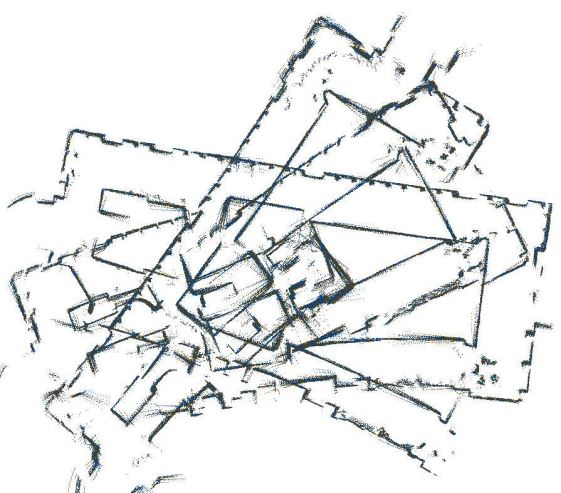
\includegraphics[width=1\linewidth]{mapeo_malo.jpg}
		\caption{Mapeo de entorno utilizando información odométrica cruda.}
	\end{subfigure}
	
	\begin{subfigure}{0.5\textwidth}
		\centering
		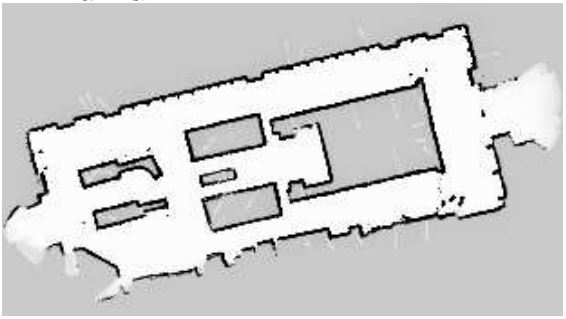
\includegraphics[width=1\linewidth]{mapeo_bueno.jpg}
		\caption{Mapeo de entorno después de fusionar la información odométrica con algoritmo.}
	\end{subfigure}
	
	\caption{Visualización del proceso de SLAM \cite{thrun_probabilistic_2005}.}
	\label{fig:SLAM}
\end{figure}
\section{Filtro de Kalman y filtro de Kalman extendido (EKF)}
El Filtro de Kalman es un algoritmo recursivo utilizado para estimar el estado de un sistema dinámico lineal en presencia de ruido. Cuenta con dos etapas principales: la etapa de predicción, donde se estima el esstao futuro del sistema utilizando el modelo dinámico y la estimación del estado actual, y la etapa de actualización, donde se ajusta la predicción con nuevas mediciones para minimizar el error en la estimación. Este filtro es ideal para sistemas lineales donde las ecuaciones del modelo y las mediciones se describen mediante relaciones lineas. Además, funciona bajo el supuesto de que tanto el proceso como el ruido de las mediciones siguen una distribución normal gaussiana. 


Cuando el sistema no es lineal, se utiliza el Filtro de Kalman Extendido (EKF, por sus siglas en inglés), una extensión del filtro de Kalman clásico. El EKF se utiliza para estimar el estado de un sistema dinámico en presencia de ruido y no linealidades. Este algoritmo funciona iterativamente, actualizando continuamente las estimaciones del estado del sistema a medida que se reciben nuevas mediciones, utilizando una versión linealizada del modelo del sistema. Al igual que el Filtro de Kalman Clásico, el EKF opera bajo dos etapas principales: la etapa de predicción y la etapa de actualización \cite{corke_robotics_2017}. 

En la primera etapa, se predice el estado actual del sistema utilizando el modelo dinámico del mismo y el estado anterior estimado. Junto con la predicción del estado, se predice su covarianza (la incertidumbre en la estimación). En la segunda etapa, se incorporan las nuevas mediciones al estado predicho para mejorar la precisión de la estimación. Se calcula la ganancia de Kalman, que determina cuánta confianza se tiene en la estimación del estado del sistema en función de la diferencia entre las mediciones reales y las predichas por el algoritmo. Finalmente, se utiliza esta ganancia para corregir la estimación del estado del sistema utilizando las mediciones disponibles de tal manera que se minimice el error de la estimación del estado \cite{corke_robotics_2017}.

Esta técnica de estimación es especialmente útil cuando el modelo del sistema y las mediciones no son lineales, lo que lo hace adecuado para sistemas como los robots móviles. Por esta razón, el EKF se utiliza en el contexto de SLAM para estimar la posición del robot en un entorno desconocido mientras construye un mapa del mismo. Siguiendo la metodología anteriormente expuesta, el EKF estima la posición y la orientación del robot en función de las mediciones odométricas y las lecturas de los sensores. A medida que el robot se mueve, se recopilan los datos de sus sensores para crear el mapa del entorno y corregir las estimaciones anteriores de la posición y orientación del mismo. Por medio de la ganancia de Kalman se compensa el error debido a pequeñas desviaciones en la rotación de las ruedas o deslizamientos en las mismas, mejorando así la precisión de la localización del robot y el mapa generado \cite{thrun_probabilistic_2005}.

\section{\textit{Light Detection and Ranging} (LiDAR)}
Los LiDAR son sistemas de teledetección que emplean pulsos de luz láser para medir distancias. Estos dispositivos emiten, de manera individual o continua, pulsos láser dirigidos hacia el objetivo que se va a medir. Al emitir un pulso láser, un circuito interno de sincronización se activa instantáneamente. Se mide el tiempo entre la emisión del pulso láser y su retorno al receptor. Los sensores receptores, al detectar la luz láser reflejada por el objetivo detienen el contador. El número de pulsos de reloj registrados durante la fase de emisión y detección es empleado para calcular la distancia hacia el objetivo. Esta tecnología es ampliamente utilizada en mediciones topográficas para generar mapas de alta resolución del terreno o la superficie. Además, son empleados en vehículos autónomos para la detección y percepción del entorno \cite{lidar}.

Esta tecnología puede clasificarse en dos tipos principales: el escáner LiDAR de una sola línea y el escáner LiDAR multilínea. El primero se utiliza para medir distancias con precisión en una dimensión específica, mientras que el segundo combina múltiples planos de escaneo para capturar mediciones en varias direcciones simultáneamente. Este último, emite pulsos láser en varias direcciones mientras gira y es utilizado en vehículos autónomos para resolver la problemática de SLAM y ofrecer un modelado del entorno más preciso \cite{lidar}.

\begin{figure}[H]
	\centering
	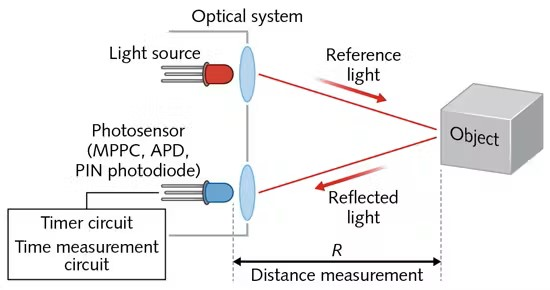
\includegraphics[width=0.65\textwidth]{lidar.jpg}
	\caption{Funcionamiento LiDAR \cite{lidar}.}
	\label{fig:lidar}
\end{figure}

\section{Sensores de distancia por tiempo de vuelo}
Como su nombre lo indica, estos sensores emplean la tecnología de \textit{Time-of-Flight} (ToF) para medir la distancia entre el sensor y un objeto. El principio de funcionamiento se basa en la velocidad de la luz. En sí, el sensor posee un emisor láser que cada cierto tiempo envía fotones que son reflejados por un objeto y detectados por el receptor. La diferencia de tiempo entre la emisión y la recepción proporciona la distancia real del objetivo en milímetros con una alta precisión. Los  sensores ToF ofrecen una rápida respuesta independientemente del tamaño y color del objeto. Son empleados en una amplia gama de aplicaciones, como sistemas de detección de obstáculos, medición de niveles de líquido, reconocimiento de gestos en cámaras y sistemas de seguridad automotriz \cite{tof}.

\section{Sensores de distancia por triangulación}
Los sensores de distancia basados en triangulación utilizan la geometría de triángulos para calcular la distancia a un objeto. En este sistema, un emisor láser proyecta un haz de luz infrarroja hacia el objeto, y la luz reflejada regresa y pasa a través de una lente que enfoca el haz en un detector, donde se registra el punto de incidencia. Este proceso forma dos triángulos similares. El primero se define por la distancia fija entre el emisor láser y el centro óptico de la lente, y la distancia desconocida al punto de reflexión en el objeto. Mientras que el segundo se establece entre el centro óptico de la lente y el plano del detector, junto con la distancia al punto donde el haz de luz reflejado incide sobre el detector.

\begin{figure}[H]
	\centering
	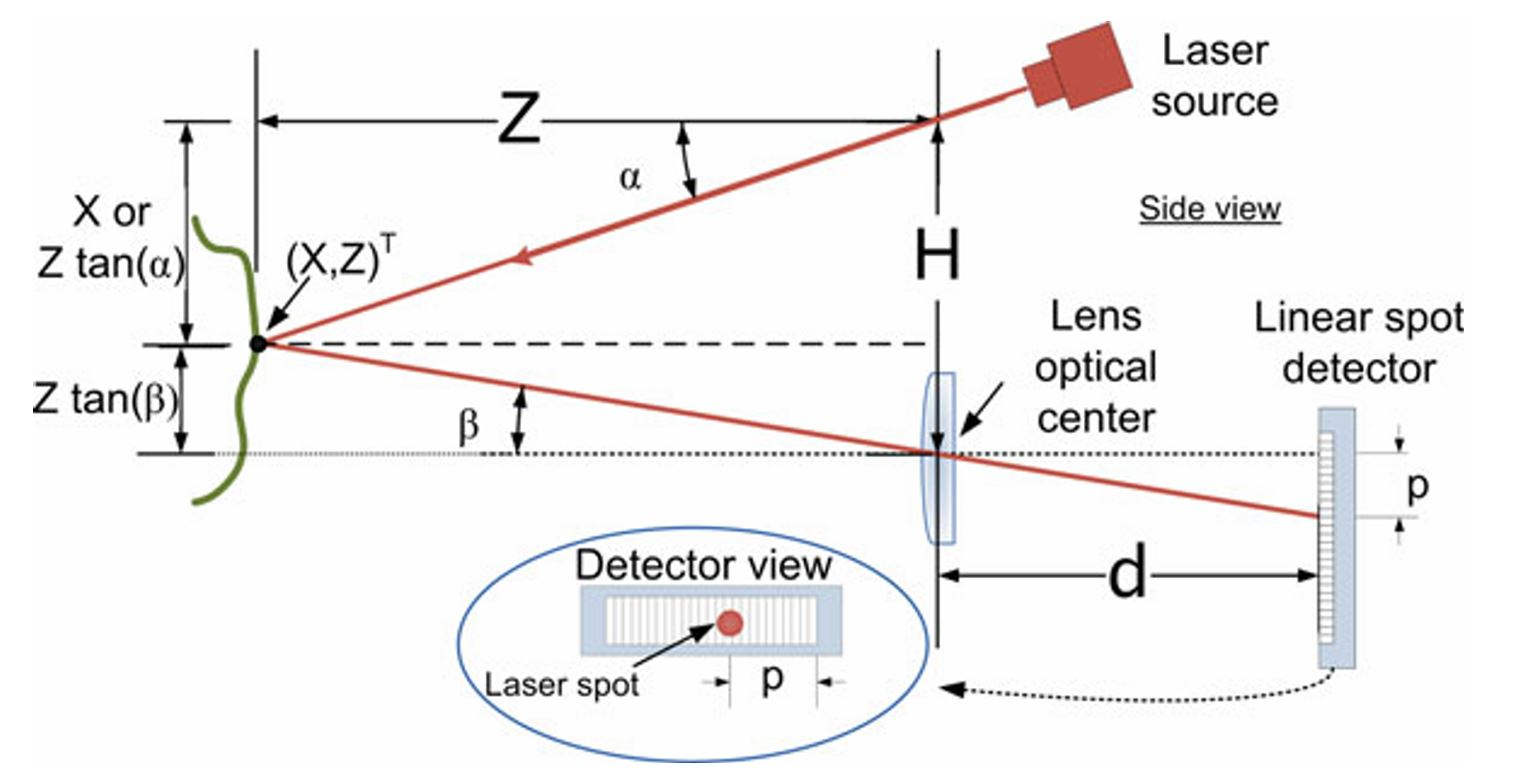
\includegraphics[width=0.75\textwidth]{triangulation.jpg}
	\caption{Diagrama esquemático de un sensor de distancia basado en triangulación. La distancia fija $H$ representa la línea base entre el emisor láser y el centro óptico de la lente, mientras que $d$ es la distancia entre la lente y el detector. El ángulo de proyección del haz láser hacia el objeto se denota como $\alpha$, y el ángulo de recolección $\beta$ se calcula en función de $d$ y la posición $p$ del punto láser en el detector. La ubicación del punto $[X,Z]^T$ se determina  a partir de la línea base $H$, el ángulo de proyección $\alpha$, y el ángulo de recolección $\beta$ \cite{drouin2020}.}
	\label{fig:triangulation}
\end{figure}

A medida que el objeto se aproxima o se aleja, el ángulo reflejado cambia, desplazando el punto de impacto en el detector. Al conocer la distancia fija entre el emisor y el detector y aplicando trigonometría, el sistema puede calcular con precisión la distancia al objeto. Esta técnica permite obtener mediciones precisas a distancias cortas y medias.


\section{Vehículo diferencial \textit{Pololu 3pi+ 32U4}}
El vehículo diferencial Pololu 3pi+ 32U4 es un pequeño robot móvil, con un diámetro nominal de 9.7 cm, manufacturado por Pololu Corporation. Está diseñado para ser un robot de tipo diferencial, por lo que emplea dos ruedas motorizadas independientes para controlar su movimiento. Esto le permite moverse con facilidad y realizar maniobras precisas al variar la velocidad de cada rueda. Una característica notable del robot es que en su núcleo se encuentra un microcontrolador AT-mega32U4 AVR de Microchip, el cual proporciona capacidad de procesamiento y control. Se puede programar utilizando el entorno de desarrollo integrado IDE de Arduino, lo que lo hace accesible para implementar distintos algoritmos de control \cite{pololu}.  

Cuenta con una variedad de sensores, que incluyen una unidad de medición inercial completa (acelerómetro, giroscopio y magnetómetro de 3 ejes), cinco sensores de reflectancia orientados hacia abajo para el seguimiento de bordes y sensores de impacto a lo largo de su cara frontal. Dispone de conexión USB para la comunicación con un ordenador, facilitando la programación del mismo en lenguajes como C o C++. Además, ofrece una serie de periféricos de expansión que permite a los usuarios personalizar y ampliar sus capacidades \cite{pololu}.
\begin{figure}[H]
	\centering
	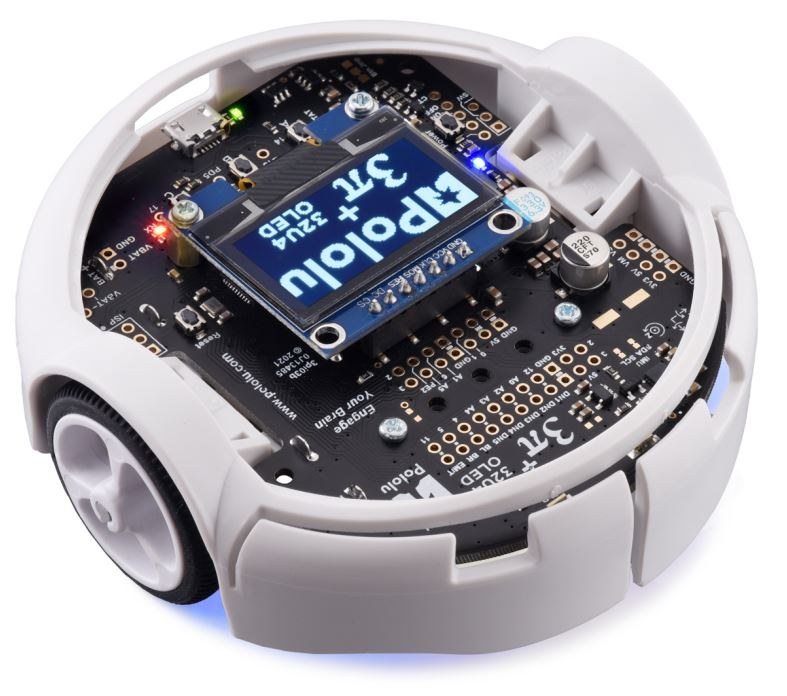
\includegraphics[width=0.5\textwidth]{pololu.jpg}
	\caption{Pololu 3pi+ 32U4 OLED Robot \cite{pololu}.}
	\label{fig:pololu}
\end{figure}

\section{\textit{Universal Asynchronous Receiver-Transmitter} (UART)}

El \textit{Universal Asynchronous Receiver-Transmitter} (UART, por sus siglas en inglés) es uno de los protocolos de comunicación más utilizados en sistemas embebidos debido a su simplicidad. Este protocolo utiliza solo dos cables para transmitir y recibir datos, y opera de manera serial y asíncrona, es decir, no requiere una señal de reloj compartida entre los dispositivos para sincronizar la transmisión de datos. En lugar de eso, la velocidad de transmisión se ajusta configurando la tasa de baudios, la cual define cuántos bits por segundo pueden ser transmitidos y recibidos entre ambos dispositivos \cite{pena_uart_nodate}.

\begin{figure}[H]
	\centering
	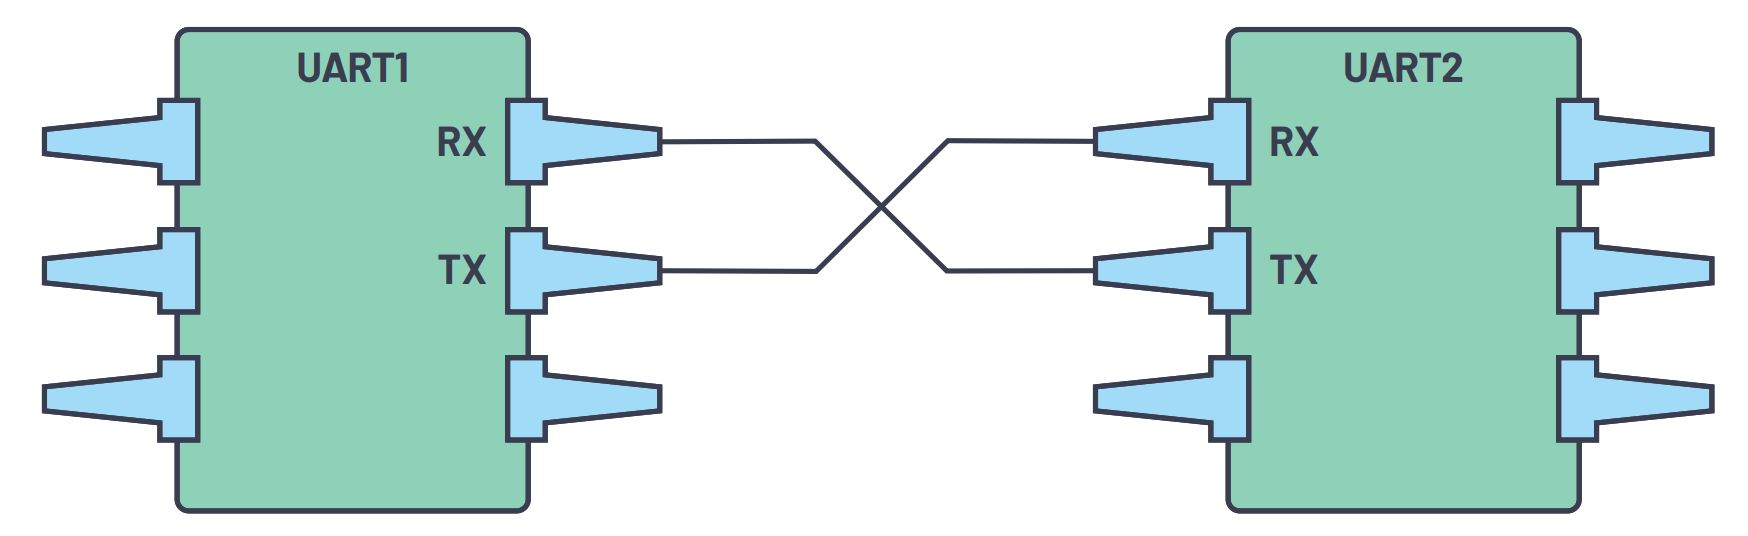
\includegraphics[width=0.7\textwidth]{uart_conexion.jpg}
	\caption{Esquema de comunicación UART entre dispositivos \cite{pena_uart_nodate}.}
	\label{fig:uart_conexión}
\end{figure}

El protocolo UART emplea dos señales principales : transmisión (Tx) y recepción (Rx) . Durante la comunicación, el UART del dispositivo convierte los datos paralelos en un flujo serial de bits, que luego se envían bit a bit a través de la línea Tx a Rx. El UART receptor recibe los datos en serie y los convierte en datos paralelos para el dispositivo receptor. Para que esta comunicación sea efectiva, ambos dispositivos deben estar configurados con la misma velocidad en baudios, lo que asegura que los bits se transmitan y reciban al mismo ritmo, sincronizando el flujo de datos \cite{campbell_basics_2016}.


Existen diferentes modos de comunicación a través de UART:
\begin{itemize}
	\item Simplex: Comunicación unidireccional. Un dispositivo seimpre actúa como transmisor y otro como receptor, sin alternar roles.
	\item Semidúplex: Comunicación bidireccional, pero no simultánea. Ambos dispositivos pueden enviar y recibir datos, pero no al mismo tiempo, se alterna entre transmisión y recepción.
	\item Dúplex completo: Comunicación bidireccional simultánea. Ambos dispositivos pueden enviar y recibir datos al mismo tiempo a través de sus respectivas líneas Tx y Rx.
\end{itemize}

Una característica importante de la comunicación UART es la implementación de una estructura de tramas (\textit{frame protocol}), que añade seguridad y robustez a la transmisión de datos. Cada trama incluye un conjunto de bits que agrupan los datos de manera estructurada con campos por encabezados, datos y verificación de errores, como el \textit{Cyclic Redundancy Check} (CRC) \cite{pena_uart_nodate}. Este protocolo asegura que los datos sean recibidos de manera confiable, y permite a los diseñadores personalizar los encabezados y finales de cada trama para adaptarse a los requisitos específicos de la aplicación. En la Figura \ref{fig:uart_frame} se muestra un ejemplo de cómo se estructura una trama UART.

\begin{figure}[H]
	\centering
	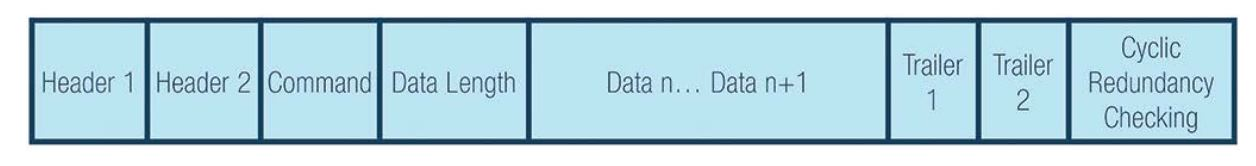
\includegraphics[width=0.8\textwidth]{uart_protocol.jpg}
	\caption{Ejemplo de protocolo de trama UART. \cite{pena_uart_nodate}.}
	\label{fig:uart_frame}
\end{figure}